\chapter{Referencial Teórico}
\label{cap:referencial}


\textit{Nesse capítulo serão apresentados os conceitos gerais do tema e o estado da arte. }
%\begin{itemize}
%\item computação paralela: modelos de computação paralela (memória compartilhada, distribuida, threads, paralelismo de dados e map reduce)
%\item map reduce
%\item ordenação
%\end{itemize}

% computação paralela
\section{Computação Pararela}

\textit{modelos de computação paralela (memória compartilhada, distribuida, threads, paralelismo de dados e map reduce)}
\section{MapReduce}

O MapReduce  é um modelo de programação paralela criado pela Google para processamento de grandes volumes de dados em \textit{clusters}. Esse modelo propõe simplificar a computação paralela e ser de fácil uso, abstraindo conceitos complexos da paralelização - como tolerância a falhas, distribuição de dados e balanço de carga - e utilizando duas funções principais: map e reduce. A complexidade do algoritmo paralelo não é vista pelo desenvolvedor, que pode se ocupar em desenvolver a solução proposta \cite{Dean:2008}. 

Esse modelo de programação é inspirado em linguagens funcionais, tendo como base as primitivas map e reduce.
Os dados de entrada são específicos para cada aplicação, e descritos pelo usuário. A saída é um conjunto de pares no formato <chave, valor>. 
A função map é aplicada aos dados de entrada e produz uma lista intermediária de pares <chave, valor>. Todos os valores intermediários associados a uma mesma chave são agrupados e enviados à função reduce. 
A função reduce é então aplicada para todos os pares intermediários com a mesma chave. A função combina esses valores para formar um conjunto menor de resultados. 
Tipicamente, há apenas zero ou um valores de saída em cada função reduce. 

%Finalmente, os pares da saída são ordenados pelo valor da chave. 

\paragraph*{Visão geral do fluxo de execução}

As chamadas da função map são distribuídas automaticamente entre as diversas máquinas através do particionamento dos dados de entrada em \textit{M} conjuntos. Cada conjunto pode ser processado em paralelo por diferentes máquinas. As chamadas reduce são distribuídas através do particionamento do conjunto intermediário de pares em \textit{R} partes. O número de partições \textit{R} pode ser definido pelo usuário. 

A Figura \ref{fig:mapreduceoverview} apresenta o fluxo de uma execução do MapReduce. A sequência de ações descrita a seguir explica o que ocorre em cada um dos passos. A numeração dos itens a seguir corresponde à numeração da figura. 



 \begin{figure}[htb]
 \centering
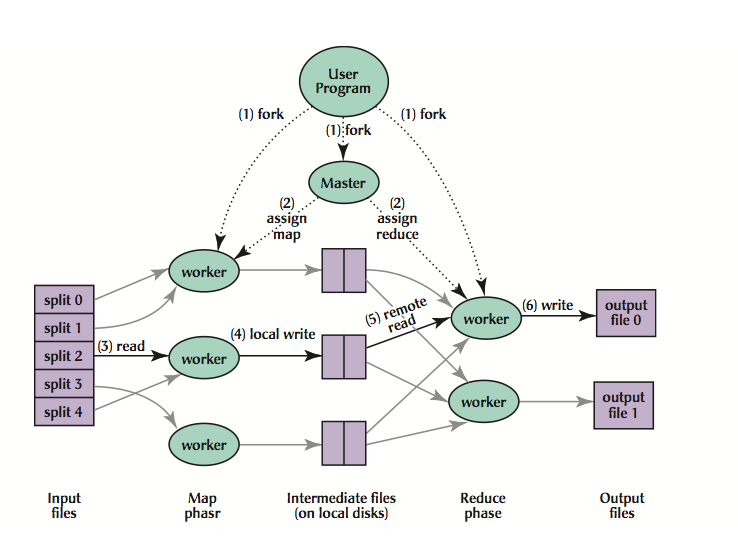
\includegraphics[scale=.65]{figuras/MapReduceOverview.png} 
\caption{Visão geral do funcionamento do modelo MapReduce.}
\label{fig:mapreduceoverview}
\end{figure}



\begin{enumerate}
\item A biblioteca MapReduce no programa do usuário primeiro divide os arquivos de entrada em M pedaços. Em seguida, iniciam-se muitas cópias do programa em um cluster de máquinas.

\item Uma das cópias do programa é especial: o mestre (master). Os demais são trabalhadores (escravos, slaves) cujo trabalho é atribuído pelo mestre. Existem M tarefas Map e R tarefas Reduce a serem atribuídas. O mestre atribui aos trabalhadores ociosos uma tarefa Map ou uma tarefa Reduce.

\item Um trabalhador que recebe uma tarefa Map lê o conteúdo do fragmento de entrada correspondente. Ele analisa pares (chave, valor), a partir dos dados de entrada e encaminha cada par para a função Map definida pelo usuário. Os pares (chave, valor) intermediários, produzidos pela função Map, são colocados no buffer de memória; 

\item Um trabalhador que recebe uma tarefa Map lê o conteúdo do fragmento de entrada correspondente. Ele analisa pares (chave, valor), a partir dos dados de entrada e encaminha cada par para a função Map definida pelo usuário. Os pares (chave, valor) intermediários, produzidos pela função Map, são colocados no buffer de memória; 

\item Periodicamente, os pares colocados no buffer são gravados no disco local, divididos em regiões R pela função de particionamento. As localizações desses pares bufferizados no disco local são passadas de volta para o mestre, que é responsável pelo encaminhamento desses locais aos trabalhadores Reduce; 

\item Quando um trabalhador Reduce é notificado pelo mestre sobre essas localizações, ele usa chamadas de procedimento remoto para ler os dados no buffer, a partir dos discos locais dos trabalhadores Map. Quando um trabalhador Reduce tiver lido todos os dados intermediários para sua partição, ela é ordenada pela chave intermediária para que todas as ocorrências da mesma chave sejam agrupadas. Se a quantidade de dados intermediários é muito grande para caber na memória, um tipo de ordenação externa é usado; 

\item O trabalhador Reduce itera sobre os dados intermediários ordenados e, para cada chave intermediária única encontrada, passa a chave e o conjunto correspondente de valores intermediários para função Reduce do usuário. A saída da função Reduce é anexada a um arquivo de saída final para essa partição Reduce; 

\item Quando todas as tarefas Map e Reduce são concluídas, o mestre acorda o programa do usuário. Neste ponto, a chamada MapReduce no programa do usuário retorna para o código do usuário.
			 		
\end{enumerate}



\subsection{Hadoop}


O Hadoop \cite{Hadoop:2010} é uma das implementações do MapReduce, um \textit{framework open source } desenvolvido por Doug Cutting em 2005 que provê o gerenciamento de computação distribuída.

Um dos principais benefícios do Hadoop é a sua capacidade de lidar com falhas (disco, processos, falhas de nós), permitindo que o trabalho do usuário possa ser concluído.

Facebook, Yahoo! e eBay utilizam o ambiente Hadoop para processar diariamente terabytes de dados e logs de eventos em seus \textit{clusters} para detecção de spam, \textit{business intelligence} e diferentes tipos de otimização \cite{Cherkasova:2011}.
 
 \begin{figure}[htb]
 \centering
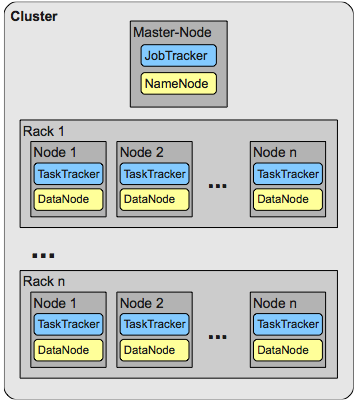
\includegraphics[scale=.65]{figuras/HadoopCluster.png} 
\caption{Visão abstrata do cluster.}
\end{figure}

\section{Ordenação Paralela}


Um grande número de aplicações paralelas possui uma fase de computação intensa, na qual uma lista de elementos deve ser ordenada com base em algum de seus atributos. Um exemplo é o algoritmo de Page Rank \cite{Page:1999} da Google: as páginas de resultado de uma consulta são classificadas de acordo com sua relevância, e então precisam ser ordenadas de maneira eficiente \cite{Kale:2010}.
No exemplo do Page Rank, o número de páginas a serem ordenadas é enorme, e elas são recolhidas de diversos servidores da Google; é uma questão fundamental escolher algoritmo paralelo com o melhor desempenho dentre as soluções possíveis.

Na criação de algoritmos de ordenação paralela, é ponto fundamental ordenar coletivamente os dados de cada processo individual, de forma a utilizar todas as unidades de processamento e minimizar os custos de redistribuição de chaves entre os processadores.
\label{cap:ordenacao}

\begin{itemize}
\item importância da ordenação paralela
\item formas de ordenação: memória e disco
\item grandes dados: apenas disco
\item grandes dados: problematização (tempo, limite de memória)
\item grandes dados: sort benchmark
\end{itemize}


\begin{itemize}
\item algoritmos de ordenação paralelos
\item funcionamento geral 
\item condições / ingredientes / limites
\item diferentes algoritmos para diferentes aplicações
\item descrição de algoritmos (e diagramas): sample sort, quick sort

\end{itemize}
\section{Algoritmos de ordenação Paralela}

\subsubsection*{Condições de implementação de algoritmos paralelos de ordenação}

\paragraph*{ $\bullet$ Habilidade de explorar distribuições iniciais parcialmente ordenadas}
Alguns algoritmos podem se beneficiar de cenários nos quais a sequência de entrada dos dados é mesma, ou pouco alterada. Nesse caso, é possível obter melhor desempenho ao realizar menos trabalho e movimentação de dados. 
Se a alteração na posição dos elementos da sequência é pequena o suficiente, grande parte dos processadores mantém seus dados iniciais e precisa se comunicar apenas com os processadores vizinhos.


\paragraph*{Movimentação dos dados}
A movimentação de dados entre processadores deve ser mínima durante a execução do algoritmo. Em um sistema de memória distribuída, a quantidade de dados a ser movimentada é um ponto crítico, pois o custo de troca de dados pode dominar o custo de execução total e limitar a escalabilidade.


\paragraph*{Balanceamento de carga} 
O algoritmo de ordenação paralela deve assegurar o balanceamento de carga ao distribuir os dados entre os processadores. Cada processador deve receber uma parcela equilibrada dos dados para ordenar, uma vez que o tempo de execução da aplicação é tipicamente limitada pela execução do processador mais sobrecarregado. 

\paragraph*{Latência de comunicação}
A latência de comunicação é definida como o tempo médio necessário para enviar uma mensagem de um processador a outro. 
Em grandes sistemas distribuídos, reduzir o tempo de latência se torna muito importante. 

\paragraph*{Sobreposição de comunicação e computação}
Em qualquer aplicação paralela, existem tarefas com focos em computação e comunicação. A sobreposição de tais tarefas permite que sejam feitas tarefas de processamento e ao mesmo tempo operações de entrada e saída de dados, evitando que os recursos fiquem ociosos durante o intervalo de tempo necessário para a transmissão da carga de trabalho. 

\subsection{Sample Sort}
\subsection{Quick Sort}

